\chapter{Background}\label{ch:background}
Developing a full featured software verification tool from end-to-end
can be a daunting task.  Bounded model checking requires several
steps.  First, the input source code must be parsed or compiled.  The
resulting abstract syntax tree (AST) must then be semantically
interpreted, and a model built of underlying program semantics.
Finally, the modeled program must be represented as an SMT query and
passed through an SMT solver.  This imposes a large barrier to entry
for prototyping a new model checking algorithm, or building a
verification tool for a new source language using existing
algorithms. 

The Boogie intermediate verification language (IVL) was designed by
Microsoft Research to alleviate the complexity of modeling new source
languages and implementing new model checking algorithms.  Boogie IVL
separates the task of modeling input program semantics from the task
of bounding and checking modeled programs.  This allows model checking
tools to take Boogie IVL files as input, rather than the input source
language.  Similarly, front-end tools can model the input program
semantics in Boogie IVL rather than being directly integrating with
the model checker.  By providing a clear, distinct interface between
the two tasks, Boogie IVL [allow for modular tool components rather
than end-to-end verification tools]. 

Due to its goal of creating an abstraction between program modeling
and model checking, Boogie IVL has been designed to be a very
low-level modeling language.  It contains support for little more than
a typing system, basic arithmetic and boolean expressions \&
statements, control flow \& procedure calls, and verification
condition specification~\cite{boogie}.  Any more complicated semantics
of the source language must be modeled using the basic set of
primitives available in Boogie IVL. 

Though the low-level nature of Boogie IVL provides the flexibility to
support a large variety of models of computation and source languages,
it requires that models be created to define the semantics of
operations available within the source language and computational
model environments.  As an example, there is no concept of a heap
within Boogie.  Because of this, a memory model must be developed that
accurately models the behavior of the heap.  A rudimentary model of
memory could use a simple, large array of integers to represent the
heap, where each element represents a word of memory, and C pointers
are simply indices into this array. 

[I don't like the phrasing/organization of this next paragraph - I
feel it highlights the Boogie verifier too much, and I don't have much
to say about the Boogie verifier] 

As the goal of Boogie IVL is to modularize model checking verifiers,
it shouldn't be surprising that there are several back-end model
checking tools that support Boogie IVL programs.  The original
back-end for Boogie IVL is a tool called Boogie.  In addition to being
a complete back-end verifier for Boogie IVL programs, it also provides
an API for parsing Boogie IVL and interfacing with SMT solvers.
[Paragraph intro sentence indicates paragraph will be talking about
several verifiers, but only discusses Boogie] 

[Where to put this paragraph?] It should be noted that there exists a
back-end verifier from Microsoft Research named Boogie.  The Boogie
program verifier provides similar functionality to the Corral program
verifier.  Hereafter, ``Boogie'' will refer to BoogiePL unless
otherwise specified. 

[Bad paragraph - gets sloppy in last few sentences]Corral is another
back-end Boogie IVL program verifier, and is a good example of how
Boogie simplifies the implementation of new model checking algorithms.
Corral leverages the Boogie verifier API to implement additional model
checking algorithms, such as the Lal/Reps sequentialization algorithm
[cite this - Reducing Concurrent Analysis Under...].  [... With this
and other algorithms, ] Corral has put considerable effort toward
providing [cutting-edge] support for analyzing concurrent programs.
As such, it was the ideal candidate to use as a back-end verifier for
the pthreads extension of SMACK. 

Though providing state of the art algorithms for checking concurrnt
programs, Corral is similar to the Boogie IVL in that it provides only
low-level support for modeling concurrency.  The Corral program
verifier provides an extension to Boogie IVL that includes a very
basic set of primitives for modeling concurrent programs.  This
extension includes the following calls: 

\begin{itemize}
\item \lstinline|async call| \emph{func}\lstinline|(|\emph{...}\lstinline|)| - Asynchronously calls \emph{func} with the parameter list \emph{'...'}
\item \lstinline|corral_atomic_begin()| - Begins an atomic block
\item \lstinline|corral_atomic_end()| - Ends an atomic block
\item \lstinline|corral_getThreadID()| - Returns the ID of the calling thread.
\item \lstinline|corral_getChildThreadID()| - Returns the ID of the thread most recently spawned in the calling procedure.
\end{itemize}

The behavior prescribed in the pthread specification [cite pthreads
specification] is much more complex than these low-level concurrency
primitives recognized by Corral.  As a result, to provide support for
the more complex pthread API, it is necessary to build a model of the
pthread API behavior using the primitives provided by Corral. 

[Transition from modeling in Boogie to SMACK][major work needed below this point]

Once the behavior of the pthread API has been accurately modeled in
Boogie, the front-end [someadjective] component must be extended to
translate pthread API calls in the input source into the Boogie IVL
model of the pthread calls. 

The SMACK project as a whole is an end-to-end C/C++ program verifier.
At its core, the SMACK executable is essentially a compiler that takes
C/C++ programs and translates them into Boogie IVL~\cite{smack}.   


The SMACK toolchain is depicted in Figure~\ref{fig:SMACKToolchain}.
SMACK as a whole is a front-end for a program verification toolchain
that features the Corral program verifier as its core back-end.  Input
C/C++ programs are given to Clang to compile and link, resulting in an
LLVM bytecode output.  This is then passed to the SMACK executable,
which translates the LLVM bytecode into a Boogie program that models
the behavior of the input C/C++ program.  The resulting Boogie program
is then passed to Corral.  Corral converts the Boogie program into an
SMT query, which is given to the Z3 SMT solver for evaluation. 

SMACK itself is essentially a compiler that takes C/C++ programs and
translates them into Boogie IVL~\cite{smack}.  This converted Boogie
code is then consumed by a static analysis tool that evaluates
verification conditions present in the original source code. 

\begin{figure}[!h]
  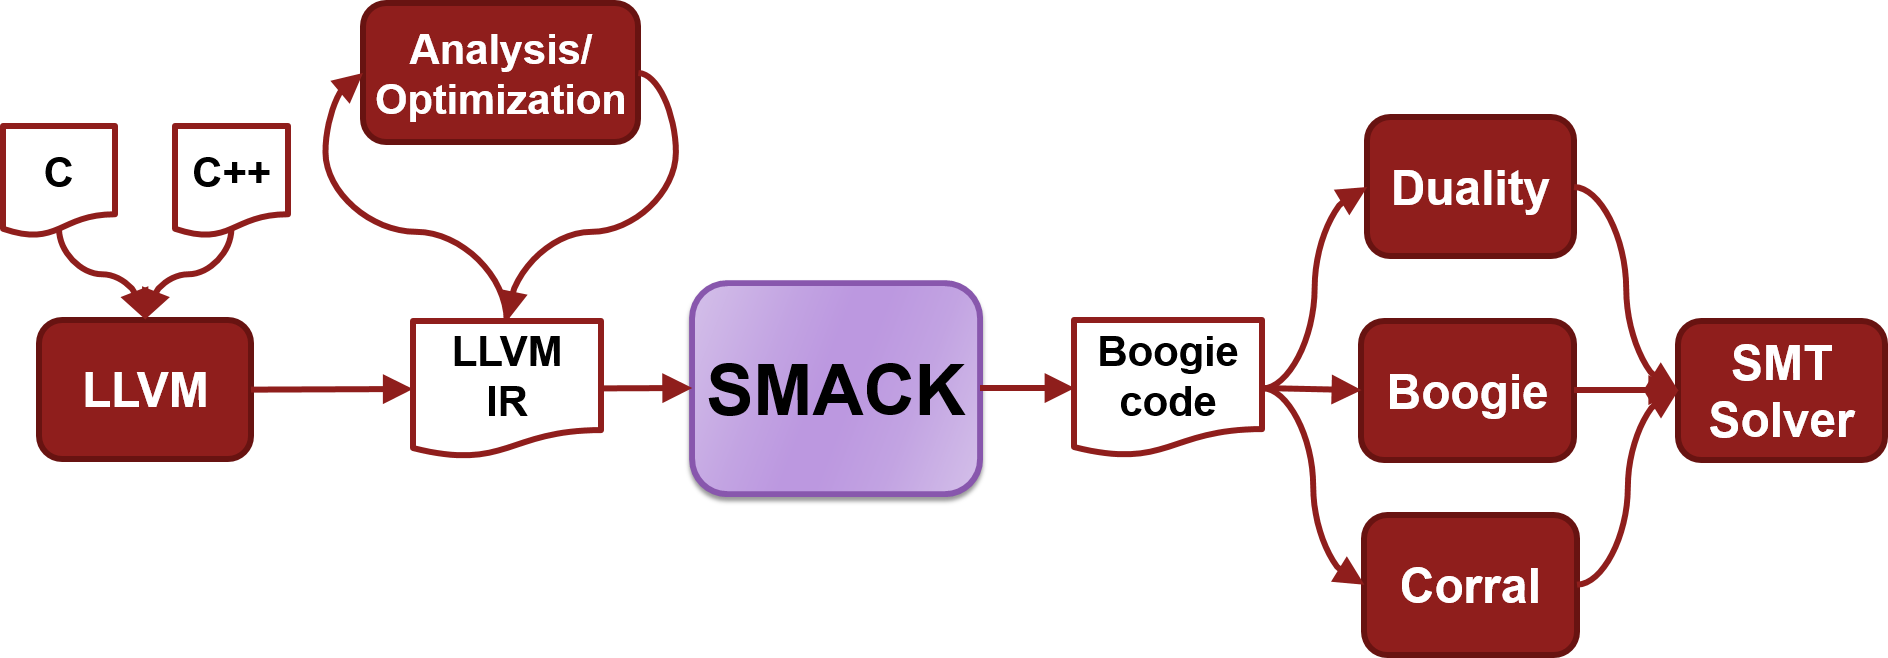
\includegraphics[width=1\textwidth]{SmackToolchain.png} 
  \caption{SMACK Toolchain}
  \label{fig:SMACKToolchain}
\end{figure}




%%% Local Variables: 
%%% mode: LaTeX
%%% TeX-master: "thesis"
%%% End: 
